\documentclass{standalone}
\usepackage{tikz}
\usepackage{xcolor}

\usetikzlibrary{decorations.pathmorphing}
\usetikzlibrary{shapes}
\usetikzlibrary{shapes.geometric}

\tikzset{
	magnetic/.style={
		fill,
		shape border rotate=0,
		isosceles triangle,
		isosceles triangle apex angle=60,
		%fill=red,
		node distance=1,
		minimum height=.1
	}
}

\tikzset{
	othermagnetic/.style={
		fill,
		shape border rotate=90,
		isosceles triangle,
		isosceles triangle apex angle=60,
		%fill=red,
		node distance=1,
		minimum height=.1
	}
}


\begin{document}
	
 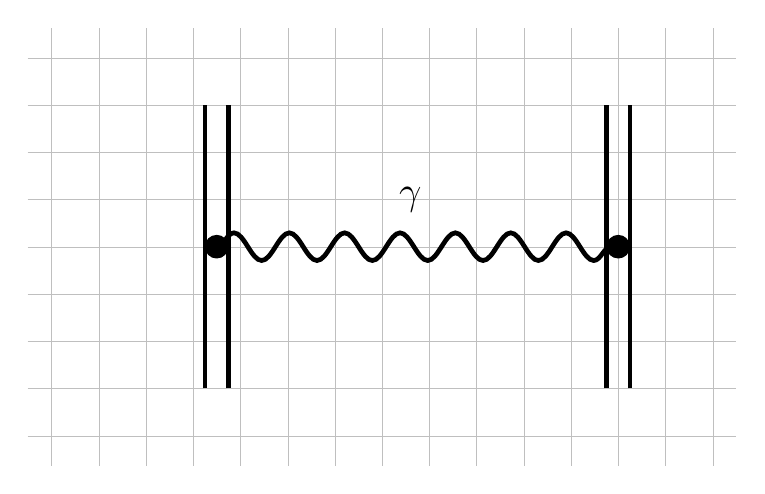
\begin{tikzpicture}[ thick,scale=3]
	% (IEI-B-1)
	\draw[gray!50,line width=0.01mm,step=0.2] (-0.5,0.073) grid (2.5, 1.927);
	\draw[line width=0.6mm] (0.3-0.05, 0.4) -- (0.3-0.05, 1.6);
	\draw[line width=0.6mm] (0.3+0.05, 0.4) -- (0.3+0.05, 1.6);
	\draw[line width=0.6mm] (2-0.05, 0.4) -- (2-0.05, 1.6);
	\draw[line width=0.6mm] (2+0.05, 0.4) -- (2+0.05, 1.6);
	\fill (0.3,1) circle (0.05);
	\draw[decorate,decoration={snake,amplitude=5,segment length=20},line width=0.6mm] (0.3,1)  -- (2,1);
	\fill (2,1) circle (0.05);
		\node at (1.1,1.2) {\fontsize{15pt}{0} $\gamma$};
	
\end{tikzpicture}\qquad
\end{document}

$ \Delta E_{NP} = \alpha \sum\limits_{\omega_L,L} \sum\limits_n \frac{\langle a |\delta V_{\rm NP}(\omega_L) | n \rangle }{\epsilon_a - \epsilon_n - {\rm sign}(\epsilon_n)\omega_L}$

